
\documentclass[18pt]{beamer}
\usepackage{graphicx}
\usepackage{amsmath}
\usepackage{amssymb}
\usepackage{mathtools}
\usepackage{caption}
\usepackage{subcaption}
\usetheme{kit}
\titleimage{titleImage}
\titlelogo{isas}
\institute{Seminar: Von Big Data zu Data Science -- Moderne Methoden der Informationsverarbeitung}

% Infos über die Präsentation
\title[Nonlinear Filtering with Homotopy Continuation]{Nonlinear Filtering with Homotopy Continuation}
\subtitle{}
\author{Marcel Hiltscher}
\date{22. Juni 2020}

% Folien
\begin{document}

% Title page
\begin{frame}
    \titlepage
\end{frame}

% Table of contents
\begin{frame}
    \frametitle{Gliederung}
    \tableofcontents
\end{frame}

\section{Motivation}
\subsection{Das System- und Messmodell}

% Content
\begin{frame}
    \frametitle{Das System- und Messmodell}
    \begin{figure}
        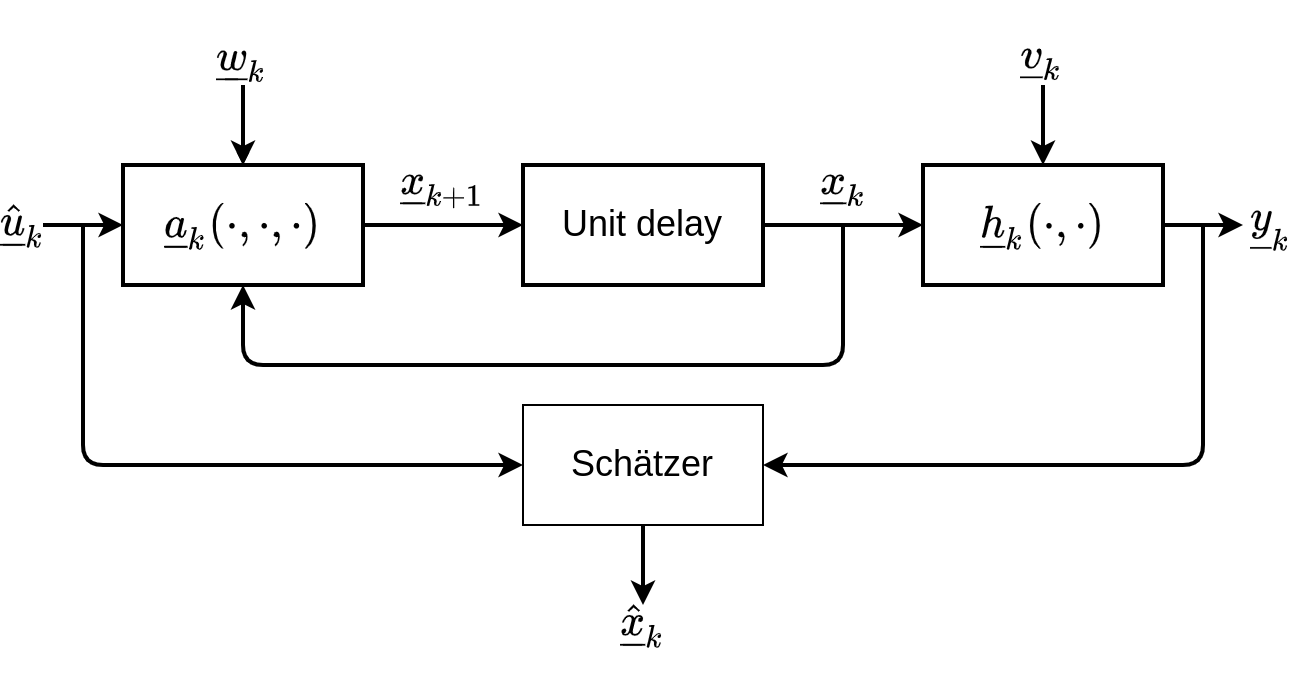
\includegraphics[scale=0.25]{pictures/system_measurment_model.png}
        \caption{Nichtlineares System- und Messungsmodell}
    \end{figure}
\end{frame}
\subsection{Filterung}

\begin{frame}
    \frametitle{Filterung}
    \begin{figure}
        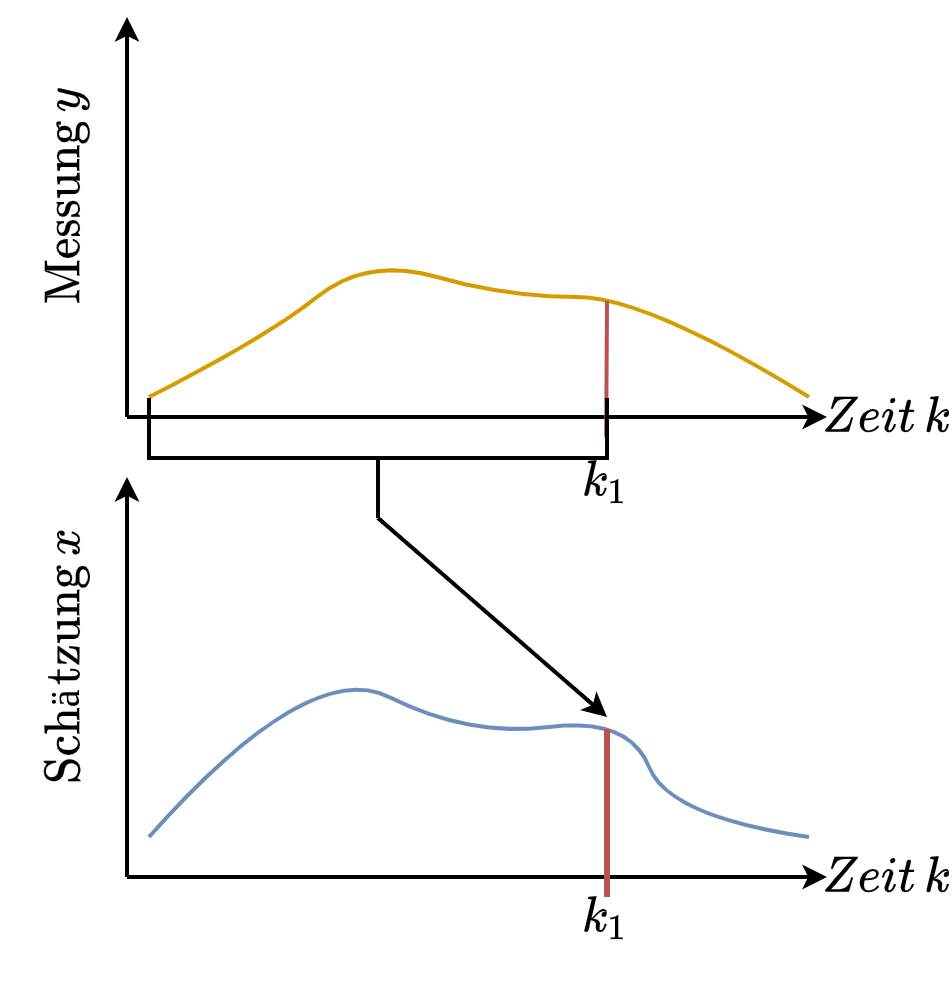
\includegraphics[scale=0.19]{pictures/filtering.png}
        \caption{Prinzip der Filterung für einen expliziten Zeitpunkt}
    \end{figure}
\end{frame}

\subsection{Herausforderung der Filterung}

\begin{frame}
    \frametitle{Herausforderung der Filterung}
    Keine closed-form Lösung für die posteriore Dichte vorhanden:   
    \begin{equation}
        f_{k+1}^{e}(\underline{x}_{k+1} \vert  \underline{Y}_{k+1}) 
        \propto  f^{L}_{k+1}(\underline{y}_{k+1} \vert \underline{x}_{k+1}) f^{p}_{k+1}(\underline{x}_{k+1} \vert \underline{Y}_{k})
    \end{equation}
    \\~\\
    \centering
    \large $\rightarrow$ Approximiere auftredende Dichte
    \begin{figure}
        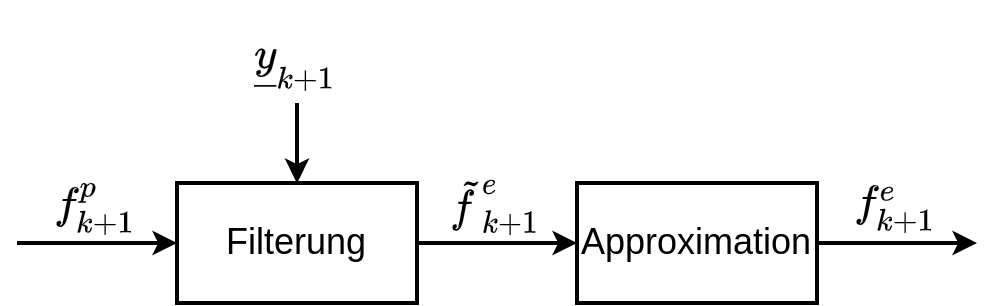
\includegraphics[scale=0.25]{pictures/approximations_vorgehen.png}
        \caption{Approximation des Filterschritts}
    \end{figure}
\end{frame}

\section{Methoden und deren Probleme}

\begin{frame}
    \frametitle{Methoden und deren Probleme}
    \begin{itemize}
        \item Parameterschätzung mithilfe einer Abweichungsmessung $G(\underline{\theta})$
        \newline
        Problem: Lokale Minima
        \newline
        \item Samplingverfahen zur Dichteschätzung
        \newline
        Problem: Sampledegenerierung
    \end{itemize}
    \vspace*{\baselineskip}
    \vspace*{\baselineskip}
    \centering 
    $\rightarrow$ Nutzung von Homotopien
\end{frame}

\section{Grundlagen der Homotopie}
\begin{frame}
    \frametitle{Grundlagen der Homotopie}
    \begin{figure}[c]
        \centering
        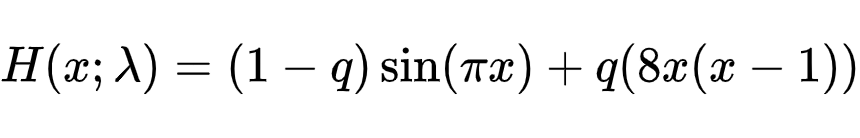
\includegraphics[scale=0.2]{pictures/homotopieoperator.png}
    \end{figure}
    \begin{figure}
        \begin{columns}
          \column{.6\linewidth}
          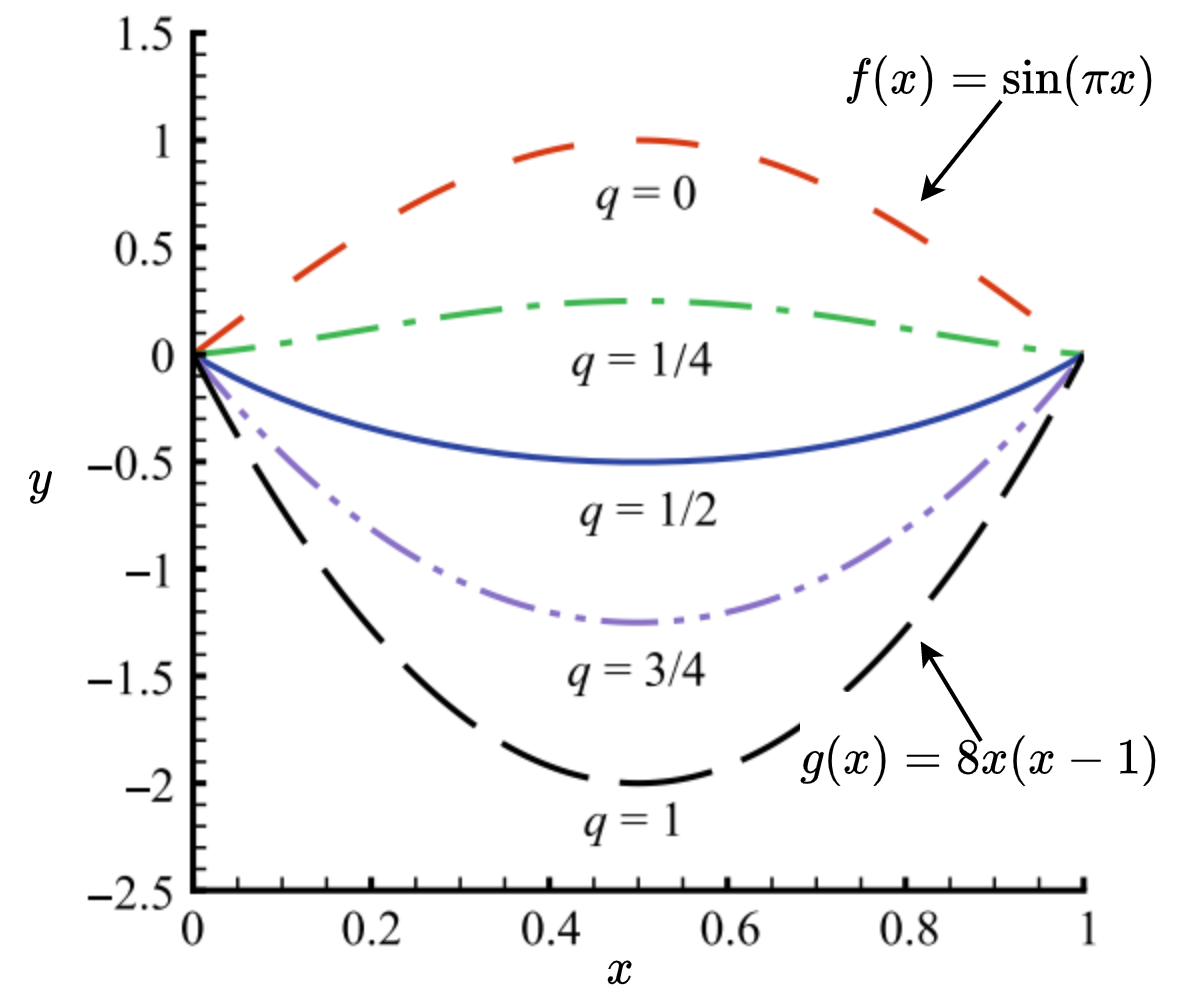
\includegraphics[width=\textwidth]{pictures/homotopieverlauf.png}
          \column{.3\linewidth}
          \caption{Homotopieverlauf nach \cite{liao2012}}
        \end{columns}
      \end{figure}
\end{frame}

\section{Homotopie und Filterung}
\begin{frame}
    \frametitle{Homotopie und Filterung}
    \begin{figure}
        \centering
        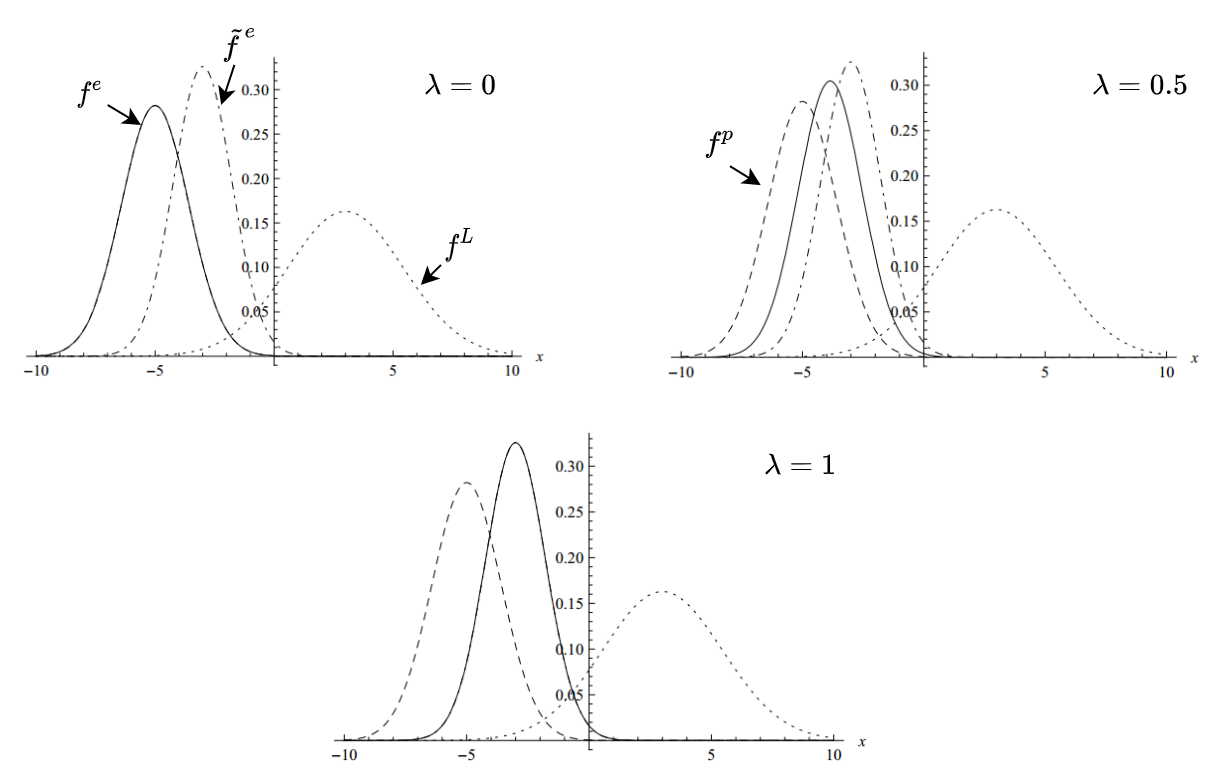
\includegraphics[scale=0.25]{pictures/homotopy_parameteroptimization.png}
        \caption{Homotopieverlauf nach \cite{hagmar2011}}
    \end{figure}
\end{frame}


\section{Parameterschätzung mit Homotopie}
\begin{frame}
    \frametitle{Parameterschätzung mit Homotopie}
    Ziel: Berechne die optimalen Parameter $\underline{\theta}$ für $f^{e}$
    \begin{enumerate}
        \item Homotopie $\tilde{f}^{e}(\underline{x},\lambda)$
        \item Approximations Dichte $f^e(\underline{x}, \underline{\theta})$ 
        \item Abweichungsmessung $G(\theta)$ zwischen $f^e(\underline{x}, \underline{\theta})$ und $\tilde{f^e}(\underline{x},\lambda)$
        \item Differentialgleichung (ODE) von der Abweichungsmessung abgeleitet
    \end{enumerate}
    \vspace{15pt}
    \centering
    Löse die ODE für bestimmtes $\lambda$ $\rightarrow$ Bekomme optimalen Parameter $\underline{\theta}$
\end{frame}



\section{Homotopie und partikel Filter}

\subsection{Idee vom Partikelfilter}
\begin{frame}
    \frametitle{Partikelfilter und Importance Sampling}
    \begin{figure}[]
        \centering
        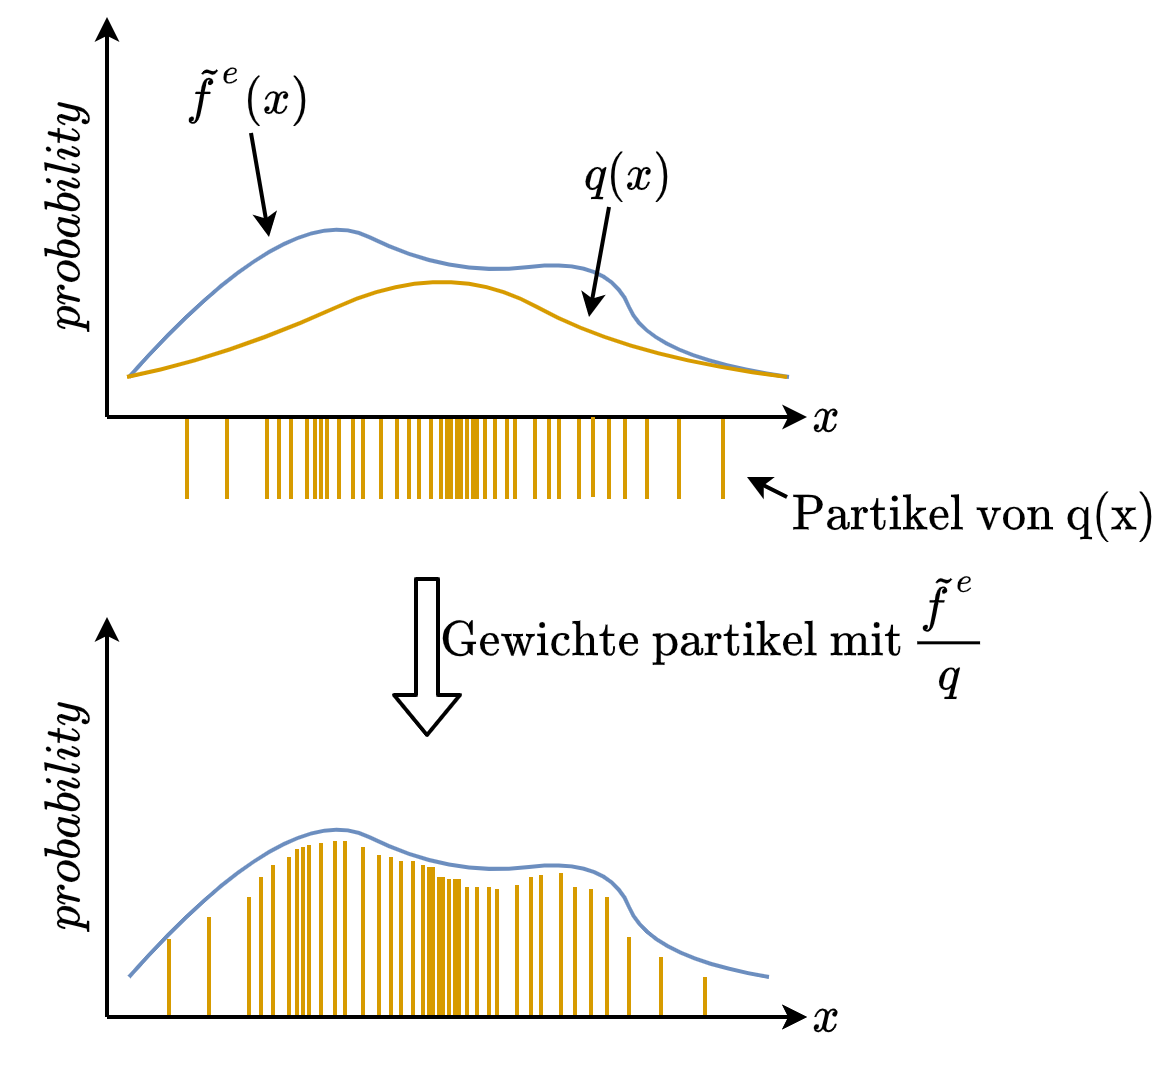
\includegraphics[scale=0.18]{pictures/particlefilter.png}
        \caption{Idee des Importance Sampling}
    \end{figure}

\end{frame}

\subsection{Partikelfilter mit Homotopie}
\begin{frame}
    \frametitle{Partikelfilter mit Homotopie}
    Erstelle mit Homotopie vorläufige Versionen der Dichte $q(x)$

    \vspace{15pt}
    Grundlegende Prozedur für die Progression $\lambda \eqslantless 1$:
    \begin{enumerate}
        \item Update die Samples mithilfe der $q(x)$
        \item Update die Gewichte mithilfe $\tilde{f}^{e}/q$
    \end{enumerate}
    \vspace{15pt}
    Mit dem letzten Schritt ($\lambda = 1$) erhält man die approximation der posterioren Dichte
\end{frame}

\section{Zusammenfassung}
\begin{frame}
    \frametitle{Zusammenfassung}

\end{frame}

% Final page
\begin{frame}{~}
	\begin{center}
		\huge{Danke für Ihre Aufmerksamkeit}
	\end{center}
\end{frame}

\begin{frame}
    \frametitle{Literatur}
    \bibliographystyle{plain}
    \bibliography{literatur.bib}
\end{frame}

\begin{frame}
    \frametitle{Zusatz}
    Homotopiegleichung für Parameterschätzung:
    \begin{equation}
        \tilde{f}^{e}(\underline{x},\lambda) = f^p(\underline{x})f^L(\underline{x})^{\lambda}
    \end{equation}
    Herleitung der ODE:
    \begin{equation}
        G_{\underline{\theta}}(\underline{\theta}, \lambda) = \frac{\partial G(\underline{\theta}, \lambda)}{\partial \underline{\theta}} = 0 
    \end{equation}
    \begin{equation}
        \begin{split}
            \frac{\partial G_{\underline{\theta}}(\underline{\theta}(\lambda),\lambda)}{\partial \lambda} &= \frac{\partial G_{\underline{\theta}}(\underline{\theta}(\lambda),\lambda)}{\partial \underline{\theta}} \frac{\partial \underline{\theta}(\lambda)}{\partial \lambda} + \frac{\partial G_{\underline{\theta}}(\underline{\theta}(\lambda),\lambda)}{\partial \lambda} \\
            &= G_{\underline{\theta}\underline{\theta}}(\underline{\theta}(\lambda),\lambda) \, \underline{\dot{\theta}}(\lambda) + G_{\underline{\theta}\lambda}(\underline{\theta}(\lambda),\lambda) 
        \end{split}
    \end{equation}
\end{frame}
\end{document}

